
In this section we provide a taxonomy of common failure modes observed in
software-defined networks. We base our analysis on conversations with
researchers at Nicira~\cite{nicira}, a startup focused on developing a network operating
system for production SDN deployments~\cite{onix}. To the best of our
knowledge 

\begin{figure}[t]
    \centering
    \begin{tabular}{ccc}
    \hspace{-5pt}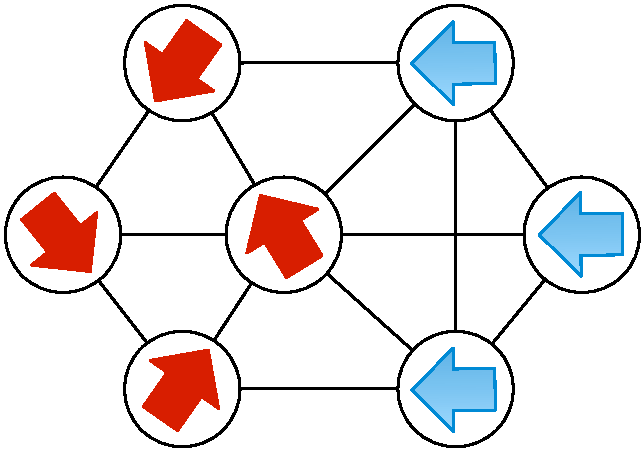
\includegraphics[width=1.3in]{../diagrams/bugs/loop.pdf}&
    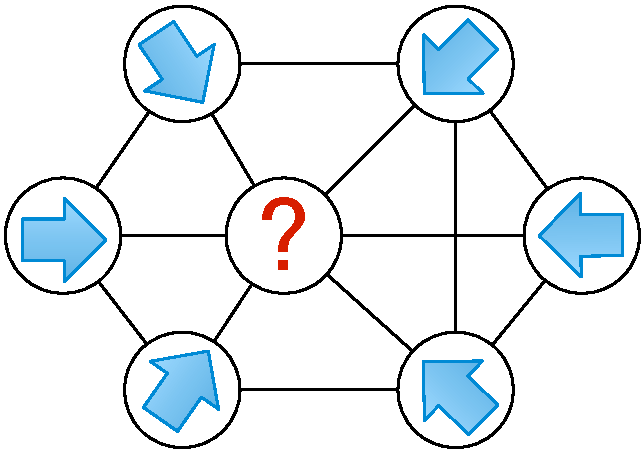
\includegraphics[width=1.3in]{../diagrams/bugs/dead_end.pdf}& \\
    {\bf (i) Loop}&{\bf (ii) Dead End}& \\
    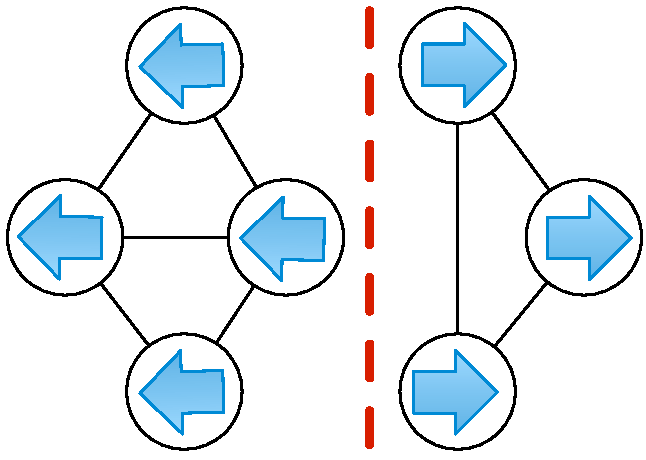
\includegraphics[width=1.3in]{../diagrams/bugs/partition.pdf}&
    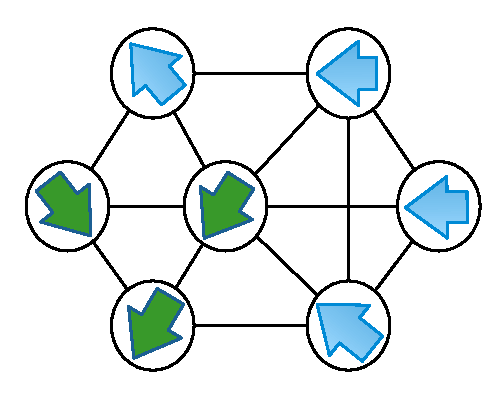
\includegraphics[width=1.3in]{../diagrams/bugs/routing_inconsistency.pdf}\\
     {\bf (iii) Partition}&{\bf (iv) Inconsistency}
    \end{tabular}
    \caption[]{\label{fig:generic_errors} Generic errors observed in
    networks.\vspace{-10pt}} 
\end{figure}

Figure \ref{fig:generic_errors} depicts a set of errors which are
common to all networks. Loops (i) are a particularly common problem which
can result in significant packet loss and congestion. Dead ends, or
`blackholes` (ii) prevent packets entering the network from reaching their
final destination. Network partitions (iii) are a related problem where
some nodes in the network are not able to reach every other node. Finally, routing
inconsistencies (iv) cause packets to be treated under multiple, conflicting policies as
they traverse the network. 

\eat{
\colin{Mention errors specific to OpenFlow? \eg overlapping flow entries. I
suppose that is really a form of routing inconsistency}
}

In addition to generic network problems, error conditions exist which are
specific to the semantics of a particular control application. For example, a network
hosting web traffic may wish to guarentee that no incoming packet arrives
at a web server without first passing through a firewall. If a hardware
failure occurs, in-flight packet might violate this guarentee. As another
example, a load-balancing application may strive to ensure that no link
remains at full utliization more than 1\% of the time. If a sudden burst of
traffic enters the network, the application may be temporarily incapable
satisfying its constraints. 

Finally, a class of errors exists where the network does not behave as the
control application intends it to. A perfectly correct control application may
tell the NOS to route to traffic destined for a particular destination
out a particular egress, for example. A bug in the NOS itself, or a byzantine
failure in a network device might cause some traffic to leave an incorrect
egress.

